\section{Presentazione della soluzione proposta (in termini generali)}

\begin{wrapfigure}{r}{.45\textwidth}
	\centering
	\vspace{-15mm}
	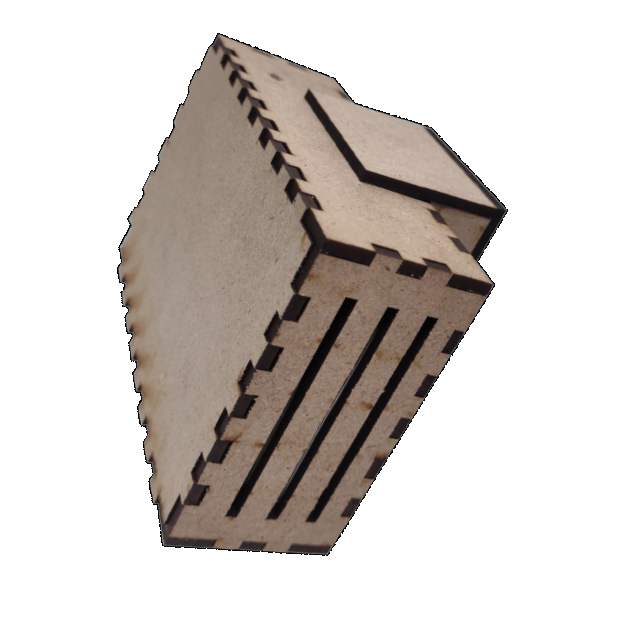
\includegraphics[width=.4\textwidth]{images/potnet.png}
	\vspace{-7mm}
	\caption{PotNet}
	\vspace{-5mm}
	\label{fig:potnet}
\end{wrapfigure}

\subsection{Descrizione generale}

La soluzione che proponiamo è \textbf{PotNet} ed è un \textbf{dispositivo intelligente che supporta gli utenti nella crescita delle proprie piante}. In figura \ref{fig:potnet} è possibile vedere un primo prototipo che mostra il principale punto di forza di PotNet: l'\textbf{adattabilità}, che ne fa un dispositivo assolutamente \textit{smart}, insieme con la facilità di utilizzo.

PotNet, infatti, si infila nei vasi comunemente presenti nelle abitazioni e, una volta a contatto con il terriccio, inizia a \textbf{monitorare i parametri vitali della pianta} che controlla.
Dopo averlo connesso ad internet, tramite la sua interfaccia web o grazie all'integrazione con Telegram è possibile informare PotNet su quale sia la pianta in crescita nel vaso: ha così inizio il monitoraggio e l'utente sarà avvisato nel caso in cui uno dei parametri vitali della pianta superi i valori di norma.

Quando si ha voglia, inoltre, è possibile chiedere a PotNet lo stato della sua pianta e ricevere suggerimenti per una corretta crescita.

\subsection{La regola del C$^3$}

\begin{figure}[h]
	\centering
	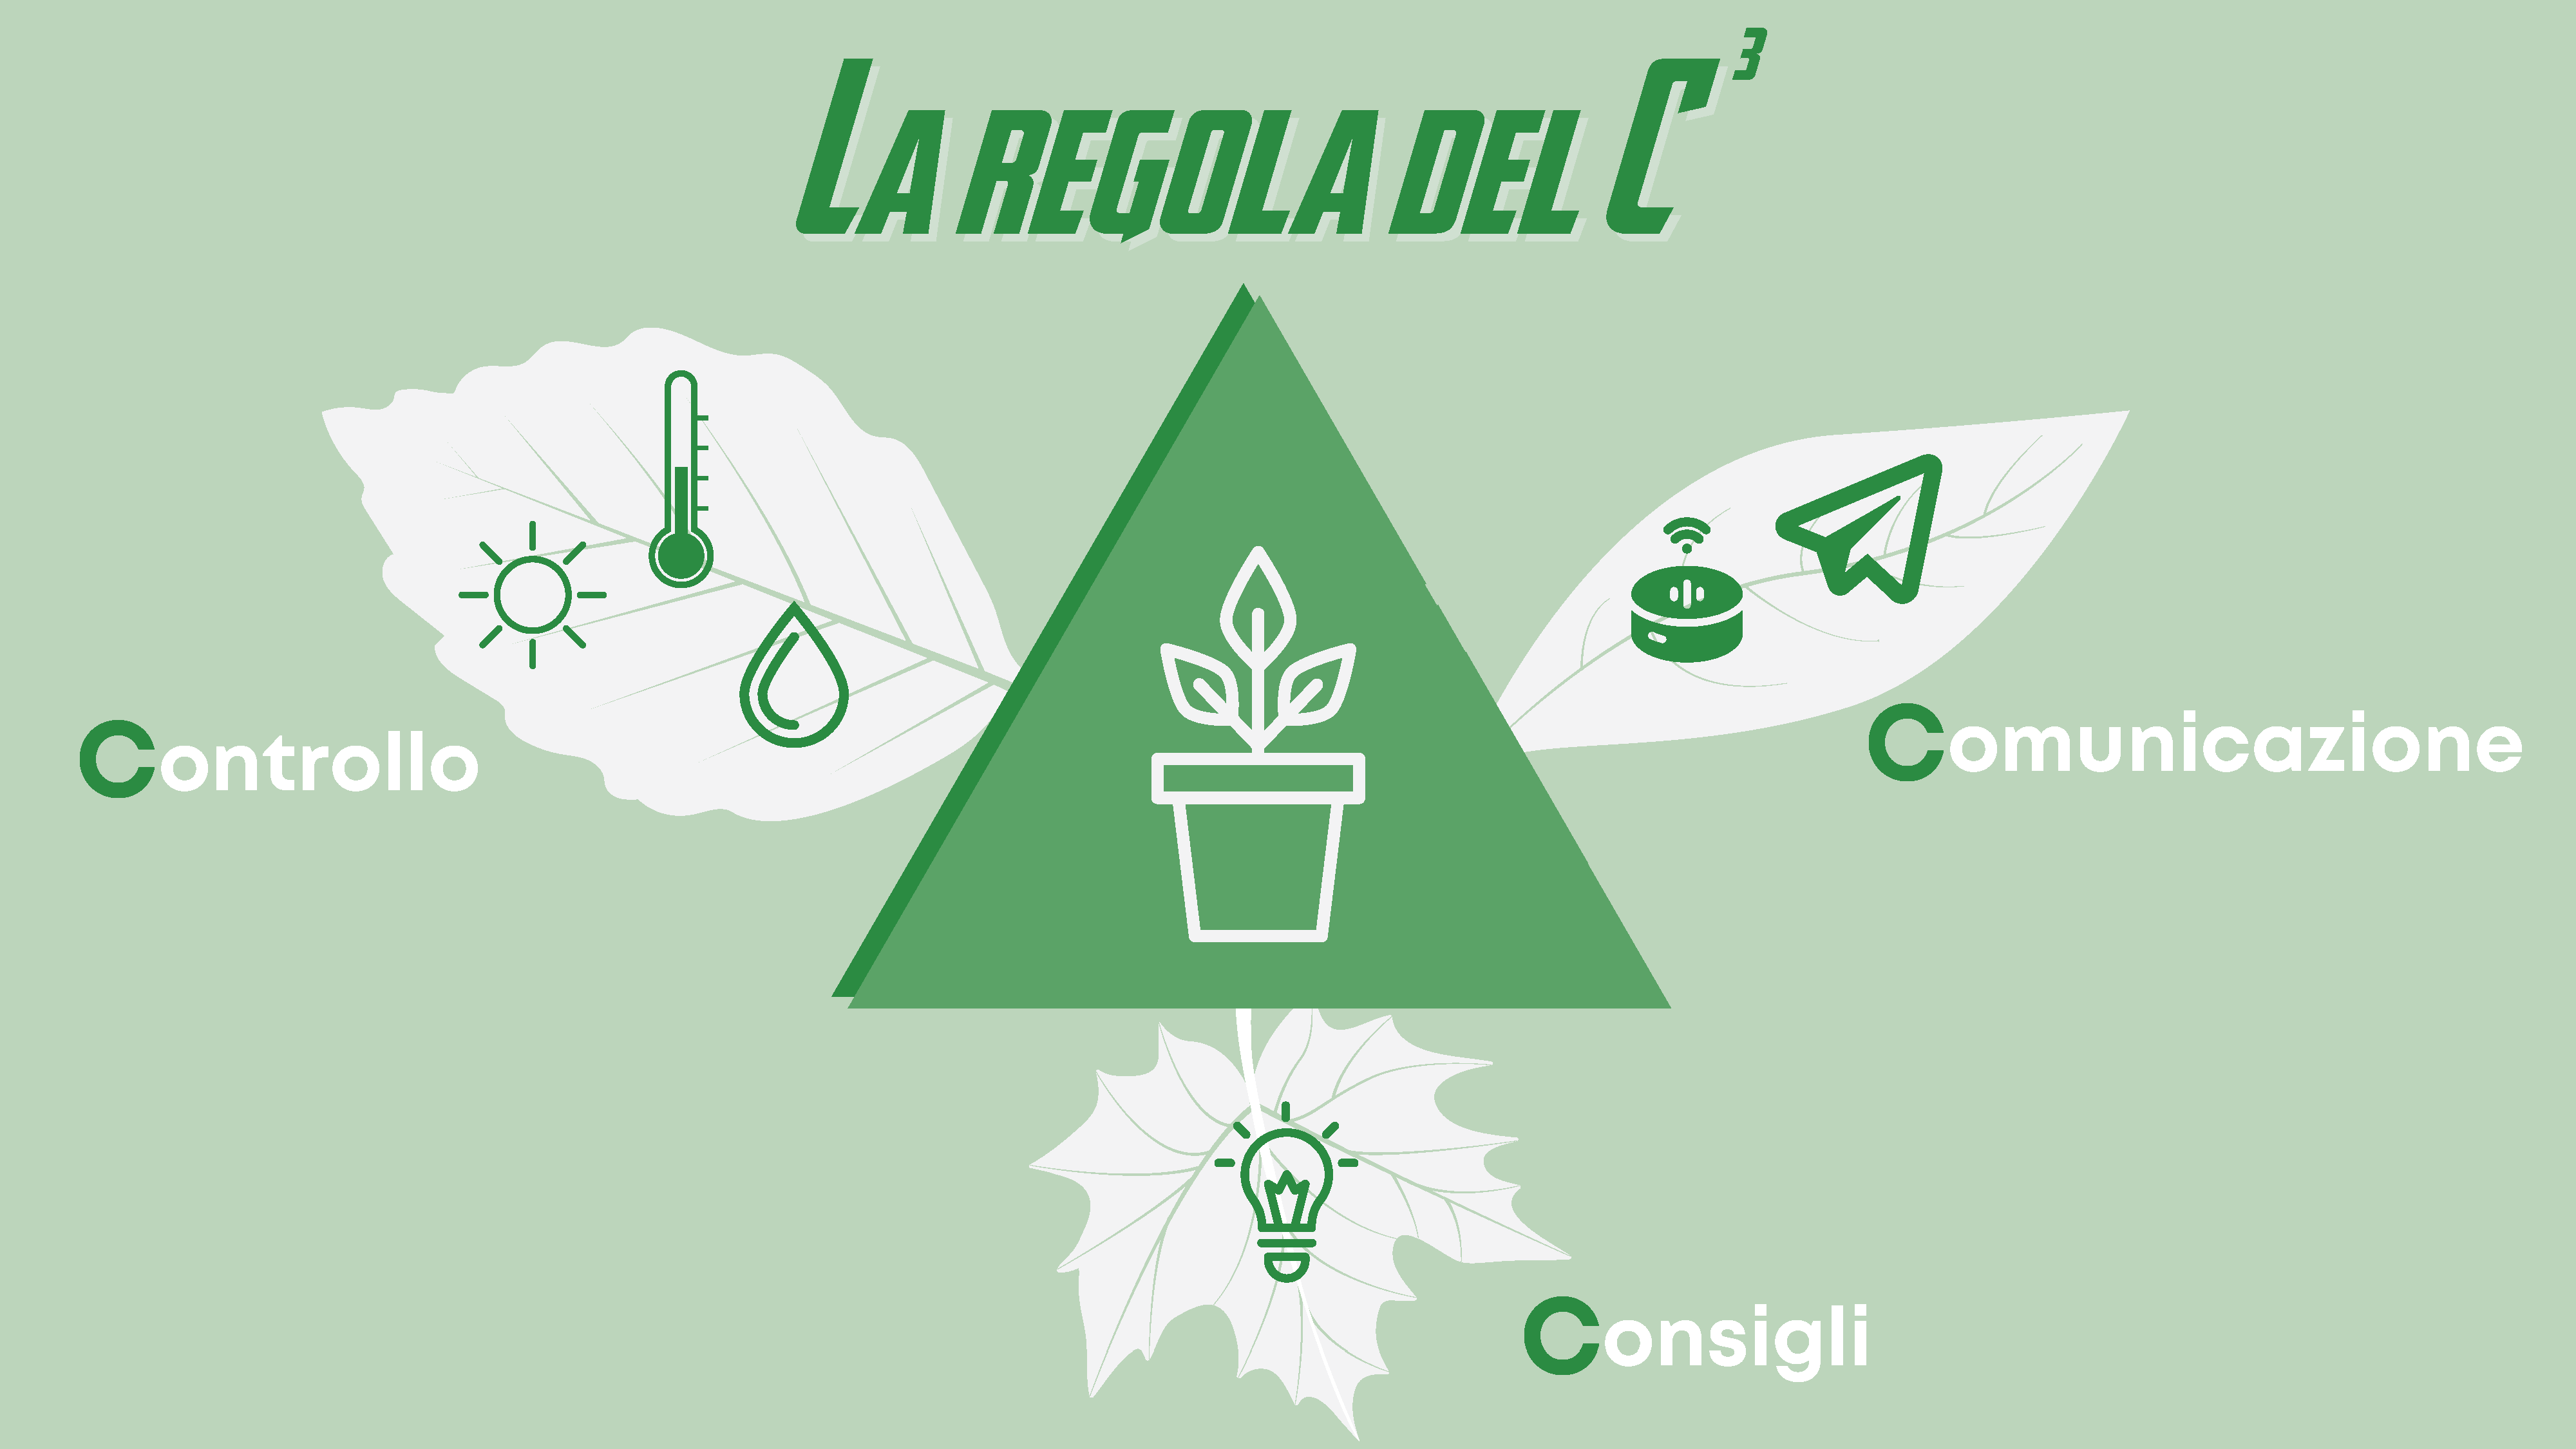
\includegraphics[width=.5\textwidth]{images/c3_rule.png}
	\caption{La regola del C$^3$}
	\label{fig:c3rule}
\end{figure}

PotNet segue la \textbf{regola del C$^3$}:
\begin{itemize}
	\item \textbf{Controllo}\\
	PotNet monitora continuamente tutti i parametri vitali della pianta e si accorge subito di qualche variazione o cambiamento significativo. Per ora, si controllano:
	\begin{itemize}
		\item \textit{temperatura} dell'ambiente che circonda la pianta;
		\item \textit{umidità} del terreno;
		\item \textit{luminosità} che arriva alla pianta.
	\end{itemize}
	
	\item \textbf{Consigli}\\
	PotNet mostra all'utente alcuni consigli personalizzati utili per trattare correttamente la sua pianta in modo che questi possa prendersene cura nel migliore dei modi.
	
	\item \textbf{Comunicazione}\\
	PotNet comunica con l'utente grazie a \textit{Telegram}, inviando immediatamente delle notifiche qualora sia richiesto l'intervento dell'utente (ad esempio perché il terreno è troppo asciutto e la pianta necessita di acqua). Inoltre, PotNet estende questo tipo di interazione grazie al fatto che è perfettamente integrabile con gli assistenti vocali\footnote{Nella versione prototipale di PotNet è stata scelta Alexa, ma è prevista anche l'integrazione con l'assistente vocale \textit{Google}}.
\end{itemize}

\subsection{Proposizione di valore}

\begin{figure}[h]
	\centering
	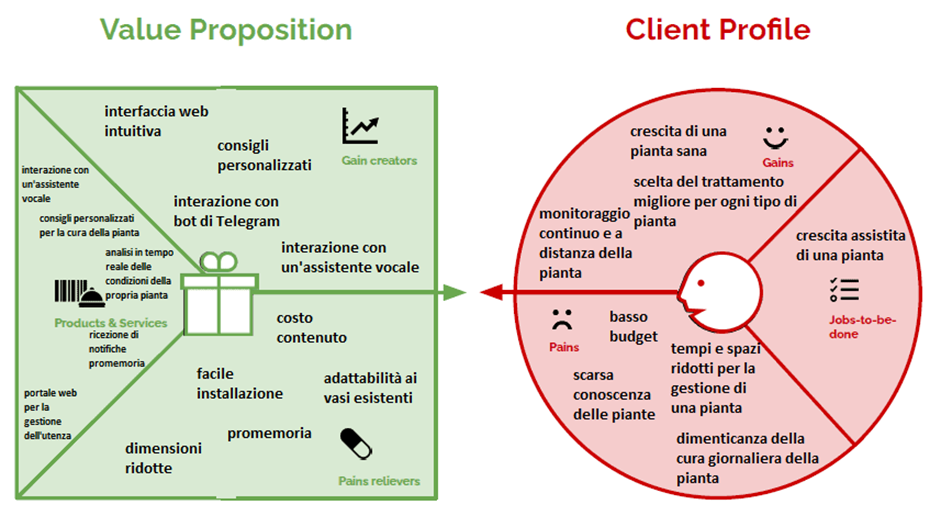
\includegraphics[width=\textwidth]{images/value_proposition.png}
	\caption{Canvas della proposizione di valore}
	\label{fig:value_proposition}
\end{figure}

La figura \ref{fig:value_proposition} mostra il \textit{canvas} della \textit{proposizione di valore} di PotNet.